% input files

\begin{center}
    \LARGE \textsc{Всеобщая тетрадь}
\end{center}

\hrule

\phantom{42}

\thispagestyle{empty}
\tableofcontents
\newpage

что-то

\subsection*{Задача 1}

Дана матрица
\begin{equation*}
	A = \frac{\sqrt{2}}{2} -\begin{pmatrix}
	    1 & \frac{3 + 4 i}{5} \\
	    \frac{3 - 4 i}{5} & -1 \\
	\end{pmatrix}
\end{equation*}
\subsubsection*{Пункт 1}
Проверим матрицу на унитарность, а именно, покажем, что $A A^* = A^* A = E$.

\newpage

% document's head
% \phantom{42}

\begin{center}
    \LARGE \textsc{Всеобщая тетрадь}
\end{center}

\hrule

\phantom{42}

\thispagestyle{empty}
\tableofcontents
\newpage

\secnum{1}{Лекции Колдунова Л.М. по современной оптики}

\sbsnum{1}{Лекция 1}
Лектор --- Л.М.Колдунов

Геометрическая оптика $\subset$  волновая оптика $\subset$ эм-оптика $\subset$ квантовая оптика.

Уравнения Максвелла:
\begin{align*}
	&\div \vc{D} = 4 \pi \rho_{\text{out}}\\
	&\div \vc{B} = 0\\
	&\rot \vc{E} = -\frac{1}{c} \frac{\partial \vc{B}}{\partial t}\\
	&\rot \bar{H} = \frac{4 \pi}{c}  \vc{j}_{\text{out}} + \frac{1}{c} \frac{\partial \vc{D}}{\partial t}\\
	&\vc{j}_{\text{out}} = 0
	\hspace{0.5 cm}
	\rho_{\text{out}} = 0\\
\end{align*}
Покрутим уравнения Максвелла:
\begin{equation*}
	\rot \rot \vc{E} = - \frac{1}{c} \frac{\partial}{\partial t} \rot \vc{B}
	\hspace{0.5 cm}
	\Rightarrow
	\hspace{0.5 cm}
	\grad \div \vc{E} = - \Delta \vc{E} = -\frac{1}{c}\mu \frac{\partial}{\partial t} \rot \vc{H} = -\frac{\varepsilon \mu}{c^2} \frac{\partial^2 \vc{E}}{\partial t^2}\\
\end{equation*}
Получаем уравнение электромагнитной волны:
\begin{equation}
	\Delta \vc{E} - \frac{\varepsilon \mu}{c^2} \frac{\partial^2 \vc{E}}{\partial t^2}
	\label{wave_eq}
\end{equation}

Получаем решение вида 
\begin{equation*}
	\vc{E} = \vc{E}_0 \exp(i \omega t - i \vc{k} \vc{r}) 
	\hspace{0.5 cm}
	\Rightarrow
	\hspace{0.5 cm}
	- k^2 \vc{E} + \frac{\varepsilon \mu}{c^2}\omega^2 \vc{E} = 0
	\hspace{0.5 cm}
	\Rightarrow
	\hspace{0.5 cm}
	\frac{\omega^2}{k^2} = \frac{c^2}{\varepsilon \mu}
\end{equation*}


\subsection*{Уравнение Эйконала}
Имеем постулаты геометрическо оптики:
\begin{enumerate}
	\item Свет распространяется в виде лучей; 
	\item Среда характеризуется показателем преломления $n$: $c_{\text{среды}} = c/n$;
	\item $\int n d l \to \text{min}$.
\end{enumerate}
\begin{to_def}
	\textit{Оптическим путём} назовём $S = \int_A^B n(\vc{r}) d l$	
\end{to_def}

Найдём ход лучей в предположении, что $ n(\vc{r})$:
\begin{equation*}
	\Delta \vc{E} - \frac{n^2}{c^2} \frac{\partial^2 \vc{E}}{\partial t^2} = 0,
	\hspace{1 cm}
	E(\vc{r}, t) = a(\vc{r}) \exp(i k_o \underbrace{\Phi(\vc{r})}_{\text{Эйконал}} - i \omega t).
\end{equation*}
Взяв $\vc{E}$ одномерным посчитаем в лоб лапласиан:
\begin{equation*}
	\Delta E = \Delta a \exp() - a (\vc{r}) k_0^2 |\grad \Phi|^2 \exp() + i (2 k_0 (\grad a, \grad \Phi) + k_0 a \Delta \Phi)exp()
\end{equation*}
Сначала вещественную часть:
\begin{equation*}
	 \Delta a \exp() - a (\vc{r}) k_0^2 |\grad \Phi|^2 \exp() + \frac{\omega^2}{c^2}n^2 a \exp() = 0
	 \hspace{0.5 cm}
	 \Rightarrow
	 \hspace{0.5 cm}
	 \boxed{
	 |\grad \Phi|^2 = \frac{1}{a k_0^2}\Delta a + n^2.}
\end{equation*}
Теперь будем считать верным предположение:
\begin{equation*}
	|\lambda \frac{\partial^2 a}{\partial x^2}| \ll |\frac{\partial a}{\partial x}|,
	\hspace{1 cm}
	|\lambda \frac{\partial a}{\partial x}| \ll a,
	\hspace{1 cm}
	\lambda \to 0.
\end{equation*}
Получаем в приближении уравнение Эйконала: 
\begin{equation}
	|\grad \Phi| =n.
\end{equation}

Выражение $\omega t - k_0 \Phi = \const$ задаёт \textit{Волновой фронт}.
\begin{equation*}
	\grad \Phi = n \vc{s},
	\hspace{1 cm}
	|\vc{s}| =1
	\hspace{1 cm}
	\frac{\partial \Phi}{\partial s} = n.
\end{equation*}
\begin{equation*}
	\omega d t - k_0 d \Phi = 0
	\hspace{0.5 cm}
	\Rightarrow
	\hspace{0.5 cm}
	\omega d t = k_0 d \Phi = k_0\frac{d \Phi }{d s} d s= k_0 n d s.
\end{equation*}

\subsection*{Принцип Ферма}
Пуст $\Phi$ --- задано однозначно: $\grad \Phi = n \vc{s}$.
Возьмём интеграл по замкнутому контуру:
\begin{equation*}
	\oint n(\vc{s}, d \vc{l}) = 0
	\hspace{0.5 cm}
	\leadsto
	\hspace{0.5 cm}
	\int_{A C B} n(\vc{s}, d \vc{l}) = \int_{A D B} n(\vc{s}, d \vc{l}).
\end{equation*}
Но $\vc{s} \cdot d \vc{l} = s d l = d l$ на $A C B$. Тогда и получим выражение, доказывающее принцип Ферма:
\begin{equation*}
	\int_{A C B} n d l = \int_{A D B} n \vc{s} \cdot d \vc{l} \leq \int_{A D B} n d l.
\end{equation*}
Приведём пару примеров: (Колдунов гнём зеркало)

\subsection*{Траектория луча}
Было соотношение, что: $m \vc{s} = \grad \Phi$. Для траектории: $\vc{s} = d \vc{r}/ d l$.
Тогда для градиента (который $d / d l$):
\begin{equation*}
	n \frac{d \vc{r}}{d l} = \grad \Phi
	\hspace{1 cm}
	\frac{d}{d l} \left(n \frac{d \vc{r}}{d l}\right) = \frac{d}{d l} \grad \Phi = \grad \frac{d \Phi}{d l} = \grad n
	\hspace{0.5 cm}
	\Rightarrow
	\hspace{0.5 cm}
	\frac{d}{d l}\left(n \frac{d \vc{r}}{d l}\right) = \grad n.
\end{equation*}
Получили уравнение луча. Давайте теперь возьмём однородную среду:
\begin{equation*}
	 n = \const 
	\hspace{0.5 cm}
	\Rightarrow
	\hspace{0.5 cm}
	 \frac{d ^2 \vc{r}}{d l^2} = 0
	 \hspace{0.5 cm}
	\Rightarrow
	\hspace{0.5 cm}
	 \vc{r} = \vc{a} l + \vc{b}.	
\end{equation*}

Теперь возьмём:
\begin{equation*}
	\frac{d}{d l}(n \vc{s}) = \grad n
	\hspace{0.5 cm}
	\leadsto
	\hspace{0.5 cm}
	\vc{s} \frac{d n }{d l} + n \frac{d \vc{s}}{d l} = \nabla n
	\hspace{0.5 cm}
	\leadsto
	\hspace{0.5 cm}
	\frac{\vc{N}}{R} = \frac{1}{n} \left(\nabla n - \vc{s} \frac{ d n}{d l}\right)
\end{equation*}
Домножим последнее выражение скалярно на $\vc{N}$:
\begin{equation*}
	0 < \frac{N^2}{R} = \frac{(\vc{N}, \nabla n)}{n}
	\hspace{0.5 cm}
	\Rightarrow
	\hspace{0.5 cm}
	(\vc{N}, \nabla n) > 0
	\hspace{0.5 cm}
	\Rightarrow
	\hspace{0.5 cm}
	\text{Луч поворачивает!}
\end{equation*}

((Пример про слоистую среду))

\subsection*{Уравнение луча в параксиальном приближении}
((картинка))
\begin{equation*}
	n(y) \cos \theta(y) = n (y d y)\cos \theta(y + dy) 
	=
	\left(n(y) + \frac{d n}{d y}\Delta y \right) cos \left(\theta(y) + \frac{d \theta}{d y} \Delta y\right)=  \left(n(y) + \frac{d n}{ d y}\Delta y \right) \left(\cos \theta - \sin \theta(y) \frac{d \theta}{d y} \Delta y \right).
\end{equation*}
То есть получаем, что
\begin{equation*}
	\frac{d n}{d y} \cos \theta(y) = n(y) \sin \theta(y) \frac{d \theta}{d y}
	\hspace{0.5 cm}
	\Rightarrow
	\hspace{0.5 cm}
	\frac{1}{n} \frac{d n}{d y} = \tan \theta \frac{d \theta}{d y} = \frac{d \theta}{d x} = \frac{d^2 y}{d x^2}.
\end{equation*}

Пример параболической зависимости $n^2 = n_0^2 (1 - \alpha^2 y^2)$ 	SELFOC.
\begin{equation*}
	\alpha y \ll 1
	\hspace{1 cm}
	y_{x x}'' = \frac{1}{n_0(1 - \alpha^2 y^2)^{1/2}} \frac{d n}{d y} = \frac{- n_0 \alpha^2 y}{n_0 (1 - \alpha^2 y^2)} = - \alpha^2 y.
	\hspace{0.5 cm}
	\Rightarrow
	\hspace{0.5 cm}
	y_{xx}'' + \alpha^2 y = 0.
\end{equation*}
Такое вещество используют при создании стекловолокна, суть в том, что при заходе в канал под разными углами скорость примерно одна и та же распространения.



((забыли про мнимую часть!!!!))


\sbsnum{2}{Лекция 2}
\subsection*{Матричная оптика}

Луч можно характеризовать его координатой $y$ и углом к оптической оси $x$. То есть $\{ y_1, \theta_1\} <->\leftrightarrow \{y_1, n_1, \theta_1\}$, и $n \theta = v$. Таким образом:
\begin{equation*}
	\begin{pmatrix}
		y_2 \\ \theta_2
	\end{pmatrix}
	=
	\begin{pmatrix}
		A & B \\ C & D
	\end{pmatrix}
	\begin{pmatrix}
		y_1 & n_1 \theta_1
	\end{pmatrix}.
\end{equation*}

\subsubsection*{Матрица перемещения}
В ходе перемещения:
\begin{equation*}
	\left\{
	\begin{aligned}
		&\theta_2 = \theta_1\\
		&y_2 = y_1 + l \theta_1
	\end{aligned}
	\right.
	\hspace{1 cm}
	\Rightarrow
	\hspace{1 cm}
	T = \begin{pmatrix}
		1 & l \\
		0 & 1
	\end{pmatrix}
\end{equation*}

Или же второй вариант,  который встречается в литературе:
\begin{equation*}
	\left\{
	\begin{aligned}
		&\theta_2 = \theta_1 n \\
		&y_2 = y_1 + (l/n) \theta_1 n
	\end{aligned}
	\right.
	\hspace{1 cm}
	\Rightarrow
	\hspace{1 cm}
	T = \begin{pmatrix}
		1 & l/n \\
		0 & 1
	\end{pmatrix}
\end{equation*}

\subsubsection*{Матрица преломления на сферической поверхности}

Пусть луч падает из среды с показателем преломления $n_1$ в $n_2$. Запишем условие падения:
\begin{equation*}
	n_1 \beta_1 = n_2 \beta_2,
	\hspace{0.3 cm}
	\beta_1 = \theta_1 + \alpha,
	\hspace{0.3 cm}
	\beta_2 = \theta_2 + \alpha,
	\hspace{0.3 cm}
	n_1 (\theta_1 + \alpha) = n_2 (\theta_2 + \alpha),
	\hspace{0.3 cm}
	\alpha = y_1/R.
\end{equation*}
\begin{equation*}
	v_2 = v_1 + \dfrac{n_1 - n_2}{R}y_1
	\hspace{1 cm}
	\Rightarrow
	\hspace{1 cm}
	P= \begin{pmatrix}
		1 & 0 \\ -\dfrac{n_2 - n_1}{R} & 1
	\end{pmatrix}
\end{equation*}
Или ещё в литературе она может встретиться как:
\begin{equation*}
	v_2 = \frac{n_1}{n_2} \theta_1 + \frac{n_1 - n_2}{n_2 R}y_1
	\hspace{1 cm}
	\Rightarrow
	\hspace{1 cm}
	P =\begin{pmatrix}
		1 & 0 \\ -\dfrac{n_2 - n_1}{n_2 R} & \dfrac{n_1}{n_2}
	\end{pmatrix}
\end{equation*}

\subsubsection*{Общий подход}
Пусть у нас есть какая-то система, части которой мы знаем как преобразуют луч по отдельности, то есть все матрицы преобразований знаем. Получаем матричное выражение с перемножением матриц:
\begin{equation*}
	M_3 M_2 M_1 \vc{a} = \vc{b}
	\hspace{0.5 cm}
	\Rightarrow
	\hspace{0.5 cm}
	\vc{a} = M_1^{-1} M_2^{-1}  M_3^{-1} \vc{b} =
	\begin{pmatrix}
		A & B \\ C & D
	\end{pmatrix}.
\end{equation*}
По факту теперь имеем и какую-то матрицу в которой очень хочется понять значение её коэффициентов.
\begin{enumerate}
	\item  $D = 0$. Означает, что луч у нас идёт в фокальной плоскости.
	\item $B = 0$. Тогда наша изображение: $y_2 = A y_1$. Так называемые \textit{сопряженные плоскости}. И $A$ называется коэффициентом \textit{поперечного увеличения}.
	\item $C = 0$. Тогда наша изображение: $y_2 = B \theta_1$. $D$ в этом случае называется коэффициентом. Тако	случай называется телескопическим.
\end{enumerate}

Перейдём у примерам.
\subsubsection*{Пример 0}
Для тонкой линзы с двумя радиусами кривизны -- внешним и внутренним:
	\begin{equation*}
		\begin{pmatrix}
			1 & 0 \\ \dfrac{n-1}{n R_2} & n
		\end{pmatrix}
		\begin{pmatrix}
			1 & 0 \\ \dfrac{1-n}{n R_1} & \dfrac{1}{n}
		\end{pmatrix}
		=
		\begin{pmatrix}
			1 & 0 \\ \dfrac{n-1}{n R_2} + \dfrac{1-n}{n R_1} & 1
		\end{pmatrix}
	\end{equation*}
	В левом нижнем углу у нас стоит \textit{оптическая сила системы}: $(n-1) \left(1/R_1 - 1/R_2\right)$.

\subsubsection*{Пример 1}
\begin{equation*}
	\begin{pmatrix}
			1 & b \\ 0 & 1
	\end{pmatrix}
	\begin{pmatrix}
			1 & 0 \\ -\frac{1}{F} & 1
	\end{pmatrix}
	\begin{pmatrix}
			1 & a \\ 0 & 1
	\end{pmatrix}
	= 
	\left(
\begin{array}{cc}
 1-\frac{b}{F} & b+a \left(1-\frac{b}{F}\right) \\
 -\frac{1}{F} & 1-\frac{a}{F} \\
\end{array}
\right)
\end{equation*}
Таким образом получаем формулу линзы занулив левый верхний элемент:
\begin{equation}
	\frac{1}{a} + \frac{1}{b} = \frac{1}{F}.
\end{equation}

\subsubsection*{Задача 2 (см) файл}
Только размер предмета не как в задаче --- а $2$ мм.

Какие матрицы запишем: сначала распространяемся, потом преломляемся, и наконец снова распространяемся.
\begin{equation*}
\begin{pmatrix}
		1 & x/n \\ 0 & 1
	\end{pmatrix}
\begin{pmatrix}
		1 & 0 \\ -0.2 & 1
	\end{pmatrix}
	\begin{pmatrix}
		1 & 15 \\ 0 & 1
	\end{pmatrix}
	=
	\begin{pmatrix}
		1- \dfrac{x}{7.8} & 15 - \dfrac{x}{0.78} \\ -0.2 & -2
	\end{pmatrix}
\end{equation*}
Снова $B = 0$ и решаем уравнение: $15 - \frac{x}{0.78} = 0$, откуда $x = 11.7$ см.
Коэффициент увеличение  $A = 1 - \dfrac{11.7}{0.78} = -0.5$.

\subsubsection*{Задача 4 (см) файл}
Снова думаем --- преломляемся--распространение--преломляемся--распространяемся.
\begin{equation*}
	\left(
\begin{array}{cc}
 1 & F \\
 0 & 1 \\
\end{array}
\right).\left(
\begin{array}{cc}
 1 & 0 \\
 \dfrac{-(1-n)}{-R} & 1 \\
\end{array}
\right).\left(
\begin{array}{cc}
 1 & \dfrac{2 R}{n} \\
 0 & 1 \\
\end{array}
\right).\left(
\begin{array}{cc}
 1 & 0 \\
 -\dfrac{n-1}{R} & 1 \\
\end{array}
\right)
=
\left(
\begin{array}{cc}
\vphantom{\bigg|}
 -\dfrac{2 F (n-1)+(n-2) R}{n R} & \dfrac{-n F+2 F+2 R}{n} \\
 \vphantom{\bigg|}
 \dfrac{2-2 n}{n R} & \dfrac{2}{n}-1 \\
\end{array}
\right)
\end{equation*}
И так $A = 0$ значит $- 2 F (n-1) = R (n-2)$, откуда $F = R \frac{2-n}{2 (n-1)}$.

\subsubsection*{Задача 11 (см) файл}
На самом деле это задача из Овчинкина 1.32.
\begin{equation*}
	\left(
\begin{array}{cc}
 1 & 0 \\
 -\frac{1}{F_1} & 1 \\
\end{array}
\right).\left(
\begin{array}{cc}
 1 & l \\
 0 & 1 \\
\end{array}
\right).\left(
\begin{array}{cc}
 1 & 0 \\
 -\frac{1}{F_2} & 1 \\
\end{array}
\right)
= 
\left(
\begin{array}{cc}
 1-\frac{l}{F_2} & l \\
 -\frac{1-\frac{l}{F_1}}{F_2}-\frac{1}{F_1} & 1-\frac{l}{F_1} \\
\end{array}
\right)
=
\left(
\begin{array}{cc}
 1-l P_2 & l \\
 -P_1-\left(1-l P_1\right) P_2 & 1-l P_1 \\
\end{array}
\right).
\end{equation*}

Про увеличения: 
\begin{equation*}
	\frac{d}{d n}( (n-1)(G_1 + G_2)	- (n-1)^2 l G_1 G_2) = 0
	\hspace{0.5 cm}
	\Rightarrow
	\hspace{0.5 cm}
	(G_1 + G_2)	- 2 (n-1) l G_1 G_2 = 0
	\hspace{0.5 cm}
	\Rightarrow
	\hspace{0.5 cm}
	l = \frac{1}{2 (n-1)} \left(\frac{1}{G_1} + \frac{1}{G_2}\right)
\end{equation*}
Или же
\begin{equation*}
	l = \frac{1}{2}\left(\frac{1}{(n-1)G_1} + \frac{1}{(n-1)G_2}\right) = \frac{F_1 + F_2}{2}.
\end{equation*}


\sbsnum{3}{Лекция 3}
\subsection*{Обобщение на случай отражения}

В прошлый раз у нас было матрица $T$ \eqref{t-matrix} и матрица $P$ \eqref{p-matrix}.

\begin{figure}[htb]
	\centering
	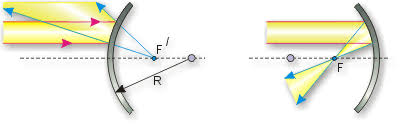
\includegraphics{img/otrazenie.png}
\end{figure}

Возьмём теперь зеркало, посмотрим на отражение для выгнутого зеркала (слева) и напишем матрицу отражения.
\begin{equation*}
	n_1 = n, n_2 = -n
	\hspace{0.5 cm}
	\leadsto
	\hspace{0.5 cm}
	R = \begin{pmatrix}
		1 & 0 \\ -\dfrac{- n -n}{R} & 1
	\end{pmatrix}
	=
	\begin{pmatrix}
		1 & 0 \\ \dfrac{2n}{R} & 1
	\end{pmatrix}
\end{equation*}
для вогнутого же (справа) заодно выпишем сразу все матрицы, которые у нас есть:
\begin{equation*}
	R = \begin{pmatrix}
		1 & 0 \\ -\dfrac{2n}{R} & 1
	\end{pmatrix}
	\hspace{1 cm}
	P= \begin{pmatrix}
		1 & 0 \\ -\dfrac{n_2 - n_1}{R} & 1
	\end{pmatrix}
	\hspace{1 cm}
	T = \begin{pmatrix}
		1 & l/n \\
		0 & 1
	\end{pmatrix}
\end{equation*}

\subsubsection*{Пример 1}
Допустим шёл луч и упал на плоскопараллельную пластину и пошёл внутри неё змейкой.
\begin{equation*}
	\begin{pmatrix}
		1 & h/n \\ 0 & 1
	\end{pmatrix}
	=
	\begin{pmatrix}
		1 & h N/n \\ 0 & 1
	\end{pmatrix}
\end{equation*}

\subsubsection*{Задача 13}
Описываем жизнь нашего  луча умножением матриц:
\begin{equation*}
	\begin{pmatrix}
		1 & 0 \\ -\dfrac{n-1}{R} & 1
	\end{pmatrix}
	\begin{pmatrix}
		1 & \dfrac{2R}{n} \\ 0 & 1
	\end{pmatrix}
	\begin{pmatrix}
		1 & 0 \\ -\dfrac{2n}{R} & 1
	\end{pmatrix}
	\begin{pmatrix}
		1 & \dfrac{2 R}{n} \\ 0 & 1
	\end{pmatrix}
	\begin{pmatrix}
		1 & 0 \\ -\dfrac{n-1}{R} & 1
	\end{pmatrix}
	= 
	\begin{pmatrix}
		\dfrac{n-4}{n} & -\dfrac{4 R}{n} \\ \dfrac{2(n-2)}{n R} & \dfrac{n-4}{n}
	\end{pmatrix}
\end{equation*}

\subsection*{Периодические оптические системы}
Пусть у нас оптическая ячейка уже после перемножения всех матриц характеризуется в итоге матрицей 2х2, с элементами $A, B, C, D$.
У периодической системы такая ячейка встречается $m$ раз:
\begin{equation*}
	\begin{pmatrix}
		y_m \\ v_m
	\end{pmatrix}
	=
	\begin{pmatrix}
		A & B \\ C & D
	\end{pmatrix}^m
	\begin{pmatrix}
		y_0 \\ v_0
	\end{pmatrix}
	\hspace{0.5 cm}
	\leadsto
	\hspace{0.5 cm}
	\begin{pmatrix}
		y_{m+1} \\ v_{m+1}
	\end{pmatrix}
	=
	\begin{pmatrix}
		A & B \\ C & D
	\end{pmatrix}^m
	\begin{pmatrix}
		y_m \\ v_m
	\end{pmatrix}
\end{equation*}
Получаем уравнения:
\begin{equation*}
\left\{
	\begin{aligned}
		&y_{m+1} = A y_m + B v_m \\
		&v_{m+1} = C y_m + D v_m
	\end{aligned}
\right.
	\hspace{0.5 cm}
	\Rightarrow
	\hspace{0.5 cm}
\left\{
	\begin{aligned}
		&v_m = \frac{y_{m+1} - A y_m}{B} 
		\hspace{0.2 cm}
		\Rightarrow
		\hspace{0.2 cm}
		v_{m+1} = \frac{y_{m+2} - A y_{m+1} }{B} \\
		&y_{m+2} - A y_{m+1} = B C y_m +D(y_{m+1} - A y_m)
	\end{aligned}
\right.
\end{equation*}
Получили уравнение на $y$:
\begin{equation*}
	y_{m+2} - (A + D) y_{m+1} + (A D - B C) y_m = 0
	\hspace{0.3 cm}
	\Rightarrow
	\hspace{0.3 cm}
	y_m = y_0 h^m
	\hspace{0.3 cm}
	\Rightarrow
	\hspace{0.3 cm}
	h^2 - (A + D)h + 1 = 0	
\end{equation*}
Заменяя $A+D = 2b$, получаем три случая на детерминант: $h_{1,2} = b \pm \sqrt{b^2 - 1}$.
\begin{enumerate}
	\item $|b|<1$: Тогда $h_{1,2} = e^{i \varphi}$ $\Rightarrow$ $y_m = \alpha_1 e^{i m \varphi} + \alpha_2 e^{- i m \varphi} = y_{\text{max}} \sin (m \varphi + \varphi_0)$.
\end{enumerate}
Заметим, что $y_m$ периодичен, только если $\varphi/2\pi$ -- рациональное число.

\subsubsection*{Пример 2}
Дана система линз: $\uparrow-d-\uparrow-d-\uparrow$. Матрицы прохождения луча:
\begin{equation*}
	\begin{pmatrix}
		1 & 0 \\ -1/F & 1
	\end{pmatrix}
	\begin{pmatrix}
		1 & d \\ 0 & 1
	\end{pmatrix}
	=
	\begin{pmatrix}
		1 & d \\ -1/F & 1 - d/F
	\end{pmatrix}
\end{equation*}
Получаем, что устойчиво когда:
\begin{equation*}
	b = \frac{2- d/F}{2}
	\hspace{0.3 cm}
	\leadsto
	\hspace{0.3 cm}
	|b|<1
	\hspace{0.3 cm}
	\leadsto
	\hspace{0.3 cm}
	0 < \frac{b}{F} < 4.
\end{equation*}
Посмотрим случаи:
\begin{enumerate}
	\item $d = F$: тогда $b = 1/2$, и тогда $b = \cos \varphi \Rightarrow \varphi = \frac{\pi}{3}$;
	\item $d = 2 F$: тогда $b=0$;
	\item $d = 0$: тогда $d = 4F$.
\end{enumerate}

\subsection*{Оптический резонатор}
Пусть у нас есть два зеркала: $\big(-L-\big)$. Матрица:
\begin{equation*}
	\begin{pmatrix}
		1 & 0 \\ 2/R_2 & 1
	\end{pmatrix}
	\begin{pmatrix}
		1 & L \\ 0 & 1
	\end{pmatrix}
	\begin{pmatrix}
		1 & 0 \\ 2/R_1 & 1
	\end{pmatrix}
	\begin{pmatrix}
		1 & L \\ 0 & 1
	\end{pmatrix}
	\hspace{0.5 cm}
	\Rightarrow
	\hspace{0.5 cm}
	b = (A + D)/2 = 2 \underbrace{\left(1 + \frac{L}{R_1}\right)}_{g_1} \underbrace{\left(1 + \frac{L}{R_2}\right)}_{g_2} - 1.
\end{equation*}
Можно рассмотреть различные типы резонаторов:
\begin{enumerate}
	\item Плоский;
	\item Симметричный конфокальный;
	\item Симметричный концентрический.
\end{enumerate}

\sbsnum{4}{Лекция 4}
 \subsection*{Оптика пучков}
 Что у нас есть. У нас есть волновое уравнение!
 \begin{equation*}
 	\nabla^2 E - \frac{\varepsilon \mu}{c^2} \frac{\partial^2 E}{\partial t^2} = 0.
 \end{equation*}
 Получаем уравнение Гельмгольца:
 \begin{equation*}
 	\nabla^2 f e^{- i \omega t} - \frac{\varepsilon \mu}{c^2} (-1) \omega^2 f e^{-i \omega t} = 0
 	\hspace{0.5 cm}
 	\Rightarrow
 	\hspace{0.5 cm}
 	\nabla^2 f + \varepsilon \frac{\omega^2}{c^2} f = 0.
 \end{equation*}
 Таким образом:
 \begin{equation}
 	\nabla^2 f + \varepsilon k_0^2 f = 0
 	\label{helmgoltz}
 \end{equation}

 Если рассматривать полну идущую от точечного источника, то вблизи мы будет ее считать \textit{сферической} чуть дальше --- \textit{параболической}, и совсем далеко --- \textit{плоской}.  

 Выберем ось $z$ на которой поместим точечный источник.
Теперь $f = \frac{A}{r} \exp(i k r)$.

На расстоянии $\rho$ от оси точка на волновом фронте лежит на $r^2 = \rho^2 + z^2$. Приблизительно в предположении $z \gg \rho$: $r \approx z + \frac{\rho^2}{2 z}$.
То есть в порядке малости выпишем:
\begin{equation*}
	\encircled{1} \, r \simeq z,
	\hspace{1 cm}
	\encircled{2} \, r \simeq \frac{2 \pi}{\lambda} (z + \frac{\rho^2}{2 z} + \ldots) = \frac{2\pi}{\lambda}z + \frac{2 \pi}{\lambda} \frac{\rho^2}{2 z}.
\end{equation*}
Второй вот порядок и называют параболическим: $f = \frac{A}{z} \exp(i k z + i k \frac{\rho^2}{2 z})$.

\subsection*{Параксиальное приближение}
Имеем ситуацию: $f (\vc{r}) = A (\vc{r}) \exp(i k z)$. Будем требовать:
\begin{equation*}
	\frac{\partial A}{\partial z}\lambda \ll A 
	\hspace{0.3 cm}
	\Rightarrow
	\hspace{0.3 cm}
	\frac{\partial A}{\partial z} \ll \frac{A}{\lambda}
	\hspace{0.3 cm}
	\Rightarrow
	\hspace{0.3 cm}
	\frac{\partial A}{\partial z} \ll A \cdot k.
\end{equation*}
\begin{equation*}
	\frac{\partial^2 A}{\partial z^2}\lambda \ll \frac{\partial A}{\partial z} 
	\hspace{0.3 cm}
	\Rightarrow
	\hspace{0.3 cm}
	\frac{\partial^2 A}{\partial z^2} \ll \frac{\partial A}{\partial z} \cdot k.
\end{equation*}
И так волновое уравнение, с заменой $k^2 = \varepsilon \omega^2/c^2$:
\begin{equation*}
	\nabla^2 f + k^2 f  = 0,
	\hspace{0.5 cm}
	\hspace{0.5 cm}
	\frac{\partial f}{\partial z} = \frac{\partial A}{\partial z} e^{i k z} + A \cdot i k e^{i k z},
	\hspace{0.5 cm}
	\hspace{0.5 cm}
	\frac{\partial^2 f}{\partial z^2} = \frac{\partial^2 A}{\partial z^2} e^{i k z} + 2 A_z' i k e^{i k z} - A k^2 e^{i k z}.
\end{equation*}
Теперь всё это в волновое уравнение:
\begin{equation*}
	\frac{\partial^2 A}{\partial z^2} + 2 \frac{\partial A}{\partial z} i k - A k^2 + \nabla^2 A + A k^2 = 0
	\hspace{0.5 cm}
	\Rightarrow
	\hspace{0.5 cm}
	\frac{\partial^2 A}{\partial z^2} + 2 \frac{\partial A}{\partial z} i k + \nabla^2 A  = 0.
\end{equation*}
И с нашем приближение получаем \textit{параксиальное уравнение Гельмгольца} (может мы где-то знак потеряли).
\begin{equation}
 	\nabla^2 A + 2 i k \frac{\partial A}{\partial z} = 0.
 	\label{parax_helm}
 \end{equation}
 Надо проверить, подставится будет ли решением уравнения сверху выражение:
 \begin{equation*}
 	f (r) = \frac{A}{z} \exp\left(-i k z - i k \frac{\rho^2}{2 z}\right)
 	\hspace{0.5 cm}
 	\Rightarrow
 	\hspace{0.5 cm}
 	f(r) = A(r) e^{- i k z},
 	\hspace{0.3 cm}
 	\hspace{0.3 cm}
 	A(r) = \frac{A}{z} \exp\left(-i k \frac{\rho^2}{2 z}\right).
 \end{equation*}
 Решение таким образом при таким $f$.	
 \begin{equation*}
 	f (r) = \frac{A}{z + i z_0} \exp\left(-i k z - i k \frac{\rho^2}{2 (z + i z_0)}\right)
 	\hspace{0.5 cm}
 	\hspace{0.5 cm}
 	z \longrightarrow q(z) = z + i z_0.
 \end{equation*}
 Тут введен $q$-параметр и \textit{Рэлеевская длина} --- $z_0$.

 Мы знаем, что  $\frac{1}{q(z)} = \frac{1}{z + i z_0} = \frac{z - i z_0}{z^2 + z_0^2}$. Подставляем:
 \begin{equation*}
 	f (r) = A \left(\frac{z}{z^2 + z_0^2} - i\frac{z_0}{z^2 + z_0^2}\right) \exp\left(- i k z - i k \frac{\rho^2}{2}\frac{z - i z_0}{z^2 + z_0^2}\right).
 \end{equation*}
 \begin{equation*}
 	f (r) = A \left(\frac{z}{z^2 + z_0^2} - i\frac{z_0}{z^2 + z_0^2}\right)
 	\exp \left( - \frac{k \rho^2}{2} \frac{z_0}{z^2 + z_0^2}\right)
 	\exp\left(- i k z - i k \frac{\rho^2 z_0}{z^2 + z_0^2}\right).
 \end{equation*}
Выпишем:	
\begin{equation*}
	- \frac{2 \pi}{2} \frac{ \rho^2 z_0}{\lambda (z^2 + z_0^2)} = i \frac{\rho^2}{\frac{\lambda}{z_0 \pi} (z^2 + z_0^2)}
	\hspace{1 cm}
	\text{обозначим: }
	W^2(z) = \frac{\lambda z_0}{\pi} (1 + \frac{z^2}{z_0^2}),
	\hspace{0.5 cm}
	R(z) = z(1 + \frac{z^2}{z_0^2}).
\end{equation*}
Тогда получаем:
\begin{equation*}
	f(r) = A \left(\frac{1}{R(z)} - i \frac{\lambda}{\pi W^2(z)}\right) \exp(- \frac{\rho^2}{W^2(z)}) \exp\left(- i k z - i k \frac{\rho^2}{2 R(z)}\right).
\end{equation*}
\begin{equation*}
	f(r) = \frac{A}{i z} \frac{W_0}{W(z)} \exp\left(-\frac{\rho^2}{W^2(z)}\right) 
	\exp\left(- i k z - i k \frac{\rho^2}{2 R(z)} + i \xi(z) \right),
\end{equation*}
где $W_0 = W(0)$, а $\xi(z) = \arctan\frac{z}{z_0}$. Обычно в первом члене ещё обозначают $A_0 = A/i z_0$.

\subsubsection*{Интенсивность}
\begin{equation*}
	I = <|\vc{S}|>_t = <\frac{c}{4 \pi} \sqrt{\varepsilon} E^2> = \frac{c n}{4 \pi}<E^2> = \frac{c n}{8 \pi} E_0^2.
\end{equation*}
И для всех будет прекрасней, для всех будет полезней не таскать коэффициент:
\begin{equation*}
	I \propto E_0^2 \hspace{0.5 cm} I \propto E^2 \hspace{0.5 cm} 
	I = E^2 \left[\frac{\text{B}^2}{\text{м}^2}\right],
\end{equation*}
сокращать на размерный коэффициент очень круто, поэтому запомним, что размерность $[I] = \frac{\text{Дж}}{\text{c cm}}$.

Таким образом со всеми предположениями:
\begin{equation*}
	I = A_0^2 \frac{W_0^2}{W^2(z)} \exp\left(- \frac{2 \rho^2}{W^2(z)}\right).
\end{equation*}
Это называется \textit{Гаусовой интенсивностью}. Читатель может построить её самостоятельно.

\subsubsection*{Мощность}
\begin{equation*}
	P = \int_0^\infty I(\rho) 2 \pi \rho d \rho = \frac{1}{2} I_0 (\pi W_0^2).
\end{equation*}
И в построенном читателями графике в предыдущем пункте если посмотреть на ширину полосы под распределением, то можно заметить, что $\rho_0 = W(z)$, в связи с чем $W(z)$ называют \textit{радиусом пучка}.

Посмотрим, что у нас с нашим радиусом творится:
\begin{equation*}
	W(z) = \sqrt{\frac{\lambda z_0}{\pi} \left(1 + \frac{z^2}{z_0^2}\right)},
\end{equation*}
если пытливый читатель построить и этот график, то он (график) пересечет $z =0$ в $W(0) = W_0 = \sqrt{\frac{\lambda z_0}{\pi}}$. Aсимптотически он будет стремиться к прямой с коэффициентом наклона: $\theta \approx \sqrt{\frac{\lambda}{\pi z_0}} = \frac{W_0}{z_0}$.

Для примера если взять лазер $\lambda_0 = 633$ нм, с $2W_0 = 2$ см, то \textit{глубина резкости} будет: $2 z_0 = 1$ км. Если же $2W_0 = 2$ мкм, то уже всё будет потоньше: $2z_0 = 1$ нм.

\sbsnum{6}{Лекция 6}
\subsection*{Уширение спектральных линий}

\subsubsection*{Естественная ширина линии}

В нашем случае это квантовое определение, которому мы прикрутим классические колёса. А именно, возьмём модель осциллятора, то есть атом излучает как:
\begin{equation*}
	\ddot{x} + 2 \gamma \dot{x} \omega_0^2 x = 0,
	\hspace{0.5 cm}
	x(0) = x_0,
	\hspace{0.5 cm}
	\dot{x}(0) = 0.
\end{equation*}
И решение соответственно:
\begin{equation*}
	x(t) = x_0 e^{- \gamma t} (\cos \omega t +\frac{\gamma}{2 \omega}\sin \omega t),
	\hspace{0.5 cm}
	\omega = \sqrt{\omega_0 - \gamma^2}.
\end{equation*}
Будем считать, что затухание у нас слабое:
\begin{equation*}
	\gamma << \omega_0 
	\hspace{0.6 cm}
	\Rightarrow
	\hspace{0.6 cm}
	x(t) = x_0 e^{-\gamma t} \cos \omega_0 t.
\end{equation*}
\begin{equation*}
	x(t) = \frac{1}{\sqrt{2 \pi}} \int_{-\infty}^{+\infty} A(\omega) e^{i \omega t} d\omega,
	\hspace{0.5 cm}
	A(\omega) = \frac{1}{\sqrt{2 \pi}} \int_{-\infty}^{+\infty} x(t) e^{-i \omega t}d t.
\end{equation*}
Имеем итого "амплитуду" преобразования Фурье:
\begin{equation*}
	A(\omega) = \frac{1}{\sqrt{2 \pi}} \int_{-\infty}^{+\infty} x_0 e^{-\gamma t} \cos \omega_0 t e^{-i \omega t}d t
	=
	\frac{1}{2\sqrt{2 \pi}} \int_{0}^{+\infty} x_0 e^{-\gamma t} e^{i(\omega_0 - \omega)t} d t
	+
	\frac{1}{2\sqrt{2 \pi}} \int_{0}^{+\infty} x_0 e^{-\gamma t} e^{i(\omega_0 + \omega)t} d t = 
\end{equation*}
\begin{equation*}
	= \frac{x_0}{2 \sqrt{2 \pi}}
	\left(
	\frac{e^{- \gamma t + i (\omega_0 - \omega)t}}{i (\omega_0 - \omega) - \gamma}
	+
	\underbrace{\frac{e^{- \gamma t + i (\omega_0 + \omega)t}}{i (\omega_0 + \omega) - \gamma}}_{\to 0}
	\right)
	\bigg|_0^\infty = \frac{x_0}{2 \sqrt{2\pi} (i (\omega_0 - \omega) - \gamma)}.
\end{equation*}
Но узнавать что-то мы ведь можем только про интесивнсоть:
\begin{equation*}
	I = \frac{x_0^2}{8 \pi ( (\omega_0 - \omega)^2 + \gamma^2 )}.
\end{equation*}
Ширина профиля $I(\omega))$ порядка $10^9$.

\subsubsection*{Доплеровское уширение}
При движении детектируемого источника на/от вас фиксируемая частота будет:
\begin{equation*}
	\omega = \omega_0 \left(1 + \frac{v_x}{c}\right)
	\hspace{1 cm}
	\Rightarrow
	\hspace{1 cm}
	\omega = \omega_0 (1 + \vc{k} \cdot \vc{v}).
\end{equation*}
То есть сколько-то атомов летит с одной скоростью на вас, сколько-то перепендикулярно вам но с большей скорости. Таким образом имеет место Гауссово распределение этих атомов по скоростям. Соотвественно больше всего тех, кто вообще не движется в проекции на вашу ось.
\begin{figure}[h]
    \centering
    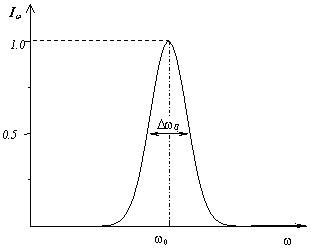
\includegraphics[width=0.3\textwidth]{img/ushir.jpg}
    %\caption{}
    %\label{fig:}
\end{figure}


Поговорим теперь про распределения:
\begin{equation*}
	v_0^2 = \frac{2 r T }{m}
	\hspace{1 cm}
	\Rightarrow
	\hspace{1 cm}
	d N =  N \exp\left( - \frac{(\omega - \omega_0)^2 c^2}{\omega_0^2 v_0^2}\right)\frac{c}{\omega_0} d \omega.
\end{equation*}

\subsubsection*{Столкновительное уширение}
\subsubsection*{Времяпролётное уширение}

\subsection*{Внутридоплеровская сперктроскопия}
\textbf{Постановка задачи:} есть атомы в коробку, которые носятся туда-сюда, а мы такие берём и посылаем пучок (ну или следим за пучок оттуда). Пусть мы нашли две линии, но из-за доплеровского уширения, если линии близки, то они неплохо так сольются, и различить их будет трудно.
\begin{figure}[h]
    \centering
    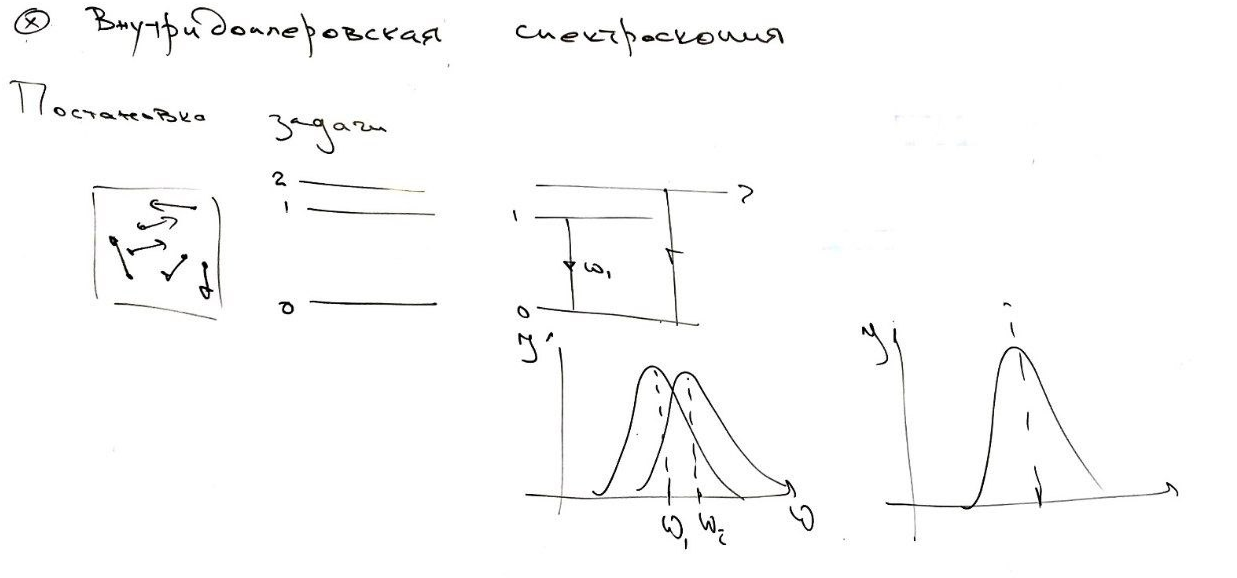
\includegraphics[width=0.7\textwidth]{img/lec_6.png}
    %\caption{}
    %\label{fig:}
\end{figure}

\subsubsection*{Квантовая механика для самых маленьких: что умеет делать электрон?}
Для сечения $\sigma$ (вероятность что-то сделать) про переходы электронов на уровни вних под/без действия внешнего излучения ответ:
\begin{itemize}
	\item электрон умеет поглощать фотончик $h \nu$;
	\item электрон умеет вынужденно излучать;
	\item электрон умеет спонтанно излучать;
	\item электрон умеет не излучать.
\end{itemize}
 
\subsubsection*{Кинематические уравнения (скоростные)}
Для двух уравнений, количество электронов на уровне: $n_1$ и $n_2$. Для характерных времен b -- bезизлучательного процесса и с -- спонтанного процесса.
\begin{equation*}
	\dot{n}_2 = - \frac{n_2}{\tau_b} - \frac{n_2}{\tau_c}
	\hspace{1 cm}
	\Rightarrow
	\hspace{1 cm}
	n_2 = n_{2 0 } \exp\left(- \frac{t}{\tau_b} - \frac{t}{\tau_c}\right).
\end{equation*}
Если есть поток фотонов $F = \frac{I}{h\nu}$, который побуждает переходить электроны и с верхнего не нижний и наоборот:
\begin{equation*}
	\dot{n}_1 = - F \sigma n_1 + F \sigma n_2 +\frac{n_2}{\tau_b}.
\end{equation*}
\begin{equation*}
	\dot{n}_2 = F \sigma n_1 - F \sigma n_2 -\frac{n_2}{\tau_b}.	
\end{equation*}
Для $n_1 + n_2 = N$:
\begin{equation*}
	\dot{n}_1 = - F \sigma n_1 + F \sigma n_2 +\frac{n_2}{\tau_b} + \frac{N}{\tau_b} - \frac{n_1}{\tau_b}
	\hspace{0.5 cm}
	\Rightarrow
	\hspace{0.5 cm}
	\dot{n}_1 + n_1 \left(2 \sigma F + \frac{1}{\tau_b}\right) = N \sigma F + \frac{N}{\tau_b}.
\end{equation*}
Таким образом:
\begin{equation*}
	n_1 = N \frac{\sigma F + \frac{1}{\tau_b}}{2 \sigma F + \frac{1}{\tau_b}} = N \frac{F + \frac{1}{`s \tau_b}}{2 F + \frac{1}{\sigma \tau_b}}.
\end{equation*}
А теперь если сказать, что то, сколько приходит и сколько уходит равны, потому как просто больше некому излучаться и поглощать, то:
\begin{equation*}
	0 = - n_1 \sigma F + n_2 \sigma F + \frac{n_2}{\tau_b}
\end{equation*}
Обозначим как что-то характерное $F_s = \frac{1}{\gamma \tau_b}$, тогда имеем 
\begin{equation*}
	n(F) = N \frac{F + F_s}{2 F + F_s}.
\end{equation*}
И введем ещё такую величину на веру: коэффициент поглощения --- $\alpha = n_1 \sigma - n_2 \sigma$. Почему так удобно:
\begin{equation*}
	d F = - (n_1 \sigma - n_2 \sigma) F d z.
\end{equation*}

Наконец. Если есть среда, которая, например поглощает красный свет, но мы будем всё больше увеличивать падающий поток, то рано или поздно атомов не хватит на поглощене и материал \textit{просветлиться}.
\begin{figure}[h]
    \centering
    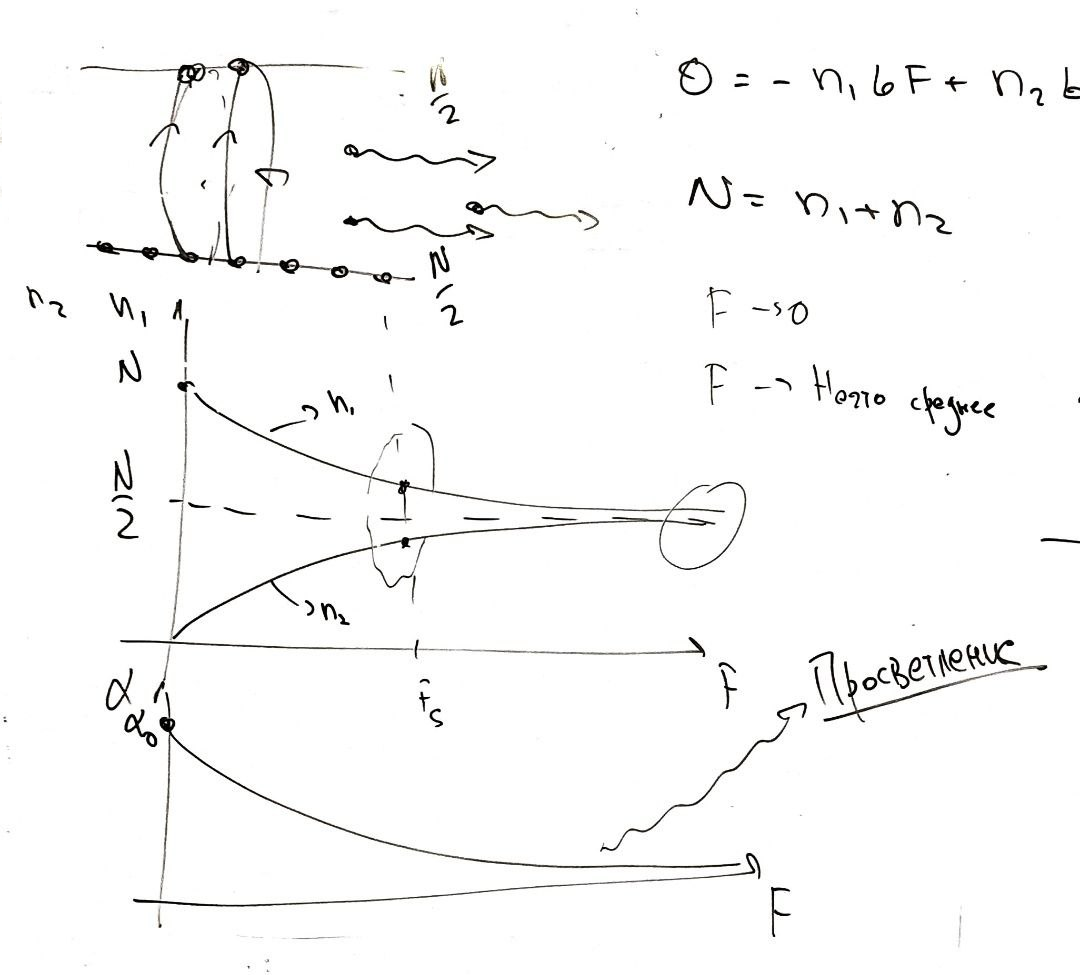
\includegraphics[width=0.4\textwidth]{img/lec_6_zerg.png}
    %\caption{}
    %\label{fig:}
\end{figure}


Напрягаемся в последний раз. Много слушаем и узнаем про провал Лэмба.

\newpage
\secnum{2}{Семинары Зябловского А.А. по теории поля}

\sbsnum{1}{Семинар по теории поля 25.03.2021}
\subsubsection*{Про мультипольное разложение}
Берем вторую пару уравнений Максвелла
\begin{equation*}
	\partial_\mu F^{\nu \mu} = - \frac{4 \pi }{c} J^\nu,
	\hspace{1 cm}
	\partial_\mu \tilde{F}^{\nu\mu} = 0.
\end{equation*}
Перепишем в терминах векторного потенциала поля:
\begin{equation*}
	\partial_\mu \left(\partial^\nu A^\mu - \partial^\mu A^\nu\right) = -\frac{4 \pi}{c} J^\nu
	\hspace{0.5 cm}
	\Rightarrow
	\hspace{0.5 cm}
	\partial^\nu \partial_\mu  A^\mu - \partial_\mu \partial^\mu A^\nu = -\frac{4 \pi}{c} J^\nu
\end{equation*}
Воспользуемся калибровкой Лоренца, то есть $\partial_\mu A^\nu = 0$. Тогда наши уравнение становится супер приятным, запишем его через оператор Даламбера:
\begin{equation*}
 	\partial_\mu \partial^\mu = \square = \frac{1}{c^2}\frac{\partial^2}{\partial t^2} - \triangle.
 \end{equation*} 
 Помня, что $J^\nu = (c \rho, \vc{J})$, получаем:
 \begin{equation}
 	\square \varphi = 4 \pi \rho
 	\hspace{1 cm}
 	\square \vc{A} = \frac{4 \pi}{c} \vc{J}
 	\label{dalamber}
 \end{equation}

Если мы говорим про электростатику, то $\rho \neq f(t)$, тогда получаем уравнение Лапласа:
\begin{equation*}
	\triangle \varphi = - 4 \pi \rho.
\end{equation*}
Решать будем с помощью функции Грина, для лапласиана и даламбертиана соответственно:
\begin{equation*}
	G(\vc{r}, \vc{r}') = \frac{-1}{4 \pi |\vc{r} - \vc{r}'|},
	\hspace{1.5 cm}
	G(\vc{r},t, \vc{r}',t') = \frac{\delta \left(t - t' - \frac{|\vc{r} - \vc{r}'|}{c}\right)}{4 \pi |\vc{r} - \vc{r}'|} 
\end{equation*}
\begin{equation}
	\varphi(x) = \int G(x, x') f(x') d x'
	\hspace{1 cm}
	\Rightarrow
	\hspace{1 cm}
	\varphi(\vc{r}) = \int \frac{\rho (\vc{r}')}{|\vc{r} - \vc{r}'|}d^3 r'
	= \frac{Q}{r} + \frac{\vc{d} \vc{r}}{r^3} + \frac{r_\alpha r_\beta D_{\alpha\beta}}{2 r^5} + \ldots
	\label{potential}
\end{equation}
Здесь введено очень удобное обозначение: 
\begin{equation*}
	\vc{d} = \int_V \rho(\vc{r})\vc{r} d^3 r \text{ --- дипольный момент.}
\end{equation*}
\begin{equation*}
	\vc{D}_{\alpha\beta} = \int \rho(r) (3 r_\alpha r_\beta - r^2 \delta_{\alpha\beta})d^3 r \text{ --- квадрупольный момент.}
\end{equation*}
Соответственно, не в нашей задаче, но в магнитостатике, аналогично:
\begin{equation*}
	\vc{A}(\vc{r}) = \int \frac{\vc{L}(\vc{r}')}{c |\vc{r} - \vc{r}'|} d^3 \vc{r}'
\end{equation*}
Проведя определенные выкладки можно получить интенсивность излучения системы зарядов в общем случае:
\begin{equation*}
	I = \frac{2 |\vc{\ddot{d}}|^2}{3 c^3} + \frac{2|\vc{\ddot{\mu}}|^2}{3 c^3} + \frac{\dddot{D}_{\alpha\beta} \dddot{D}_{\alpha\beta}}{180 c^5} + \ldots 
\end{equation*}

\sbsnum{2}{Семинар по теории поля 01.04.2021}
С прошлого семинара помним \eqref{potential}. А также выражение для величин: $\vc{d}$, $D_{\alpha\beta}$ и $Q = \int \rho(\vc{r}) d^3 \vc{r}$.
Ещё нам понадобиться выражение для октуполя:
\begin{equation*}
	O_{\alpha \beta \gamma} = \int \rho(\vc{r}) (
	15 r_\alpha r_\beta r_\gamma - 3 r_\alpha \delta_{\beta\gamma} - 3 r_\beta \delta_{\alpha \gamma} - 3 r_\gamma \delta_{\alpha\beta} r^2
	) d^3 r.
\end{equation*}
Опустим причины появления такого \textit{чудного} выражения, скажем только что октуполь войдёт в разложение для скалярного потенциала как:
\begin{equation}
	\varphi(\vc{r}) = \int \frac{\rho (\vc{r}')}{|\vc{r} - \vc{r}'|}d^3 r'
	= \frac{Q}{r} + \frac{\vc{d} \vc{r}}{r^3} + \frac{r_\alpha r_\beta D_{\alpha\beta}}{2 r^5} + \frac{O_{\alpha\beta\gamma r_\alpha r_\beta r_\gamma}}{6 r^7} + \ldots
	\label{potential8}
\end{equation}

Вот мы вводим всё новые члены разложения, но давайте же наконец посмотрим на их свойства. Начнём с квадрупольного момента:
\begin{equation*}
	D_{\alpha\beta} = D_{\beta\alpha},
	\hspace{1 cm}
	D_{\alpha\beta} \delta^{\alpha\beta} = \int \rho(\vc{r}) (3 r_\alpha r_\beta \delta^{\alpha\beta} - r^2 \delta_{\alpha\beta} \delta^{\alpha\beta}) d^3 r = 0.
\end{equation*}
Таким образом у квадрупольного момента, с получившимися ограничивающими его свойствами, существует 5 независимых элементов.

Теперь про октупольный момент. У него вообще есть 27 компонент, но сколько же из них независимы. Вариантов когда:
\begin{enumerate}
	\item  все индексы разные $O_{\alpha\beta\gamma}$ всего 6, но из-за индифферентности к перестановкам, они сводятся к 1;
	\item все индексы одинаковые $O_{\alpha\alpha\alpha}$ всега 3;
	\item Две равны и одна отлична: $O_{\alpha\alpha\beta}$ всего 18, но опять из-за перестановок их независимых остается 6.
\end{enumerate}
Итого уже сократили возможное количество независимых переменных к 10.

Теперь свёртками мы можем получить ещё связи и ещё больше сократить число независимых переменных.
\begin{equation*}
	O_{\alpha\beta\gamma}\delta^{\alpha\beta} = \int \rho(\vc{r}) (
	15 r_\alpha r_\beta r_\gamma \delta^{\alpha\beta} - 3 r_\alpha \delta_{\beta\gamma} \delta^{\alpha\beta} - 3 r_\beta \delta_{\alpha \gamma} \delta^{\alpha\beta} - 3 r_\gamma \delta_{\alpha\beta} \delta^{\alpha\beta} r^2
	) d^3 r 
	= \int \rho(\vc{r}) (15 r^2 r_\gamma - 3 r_\gamma r^2 - 3 r_\gamma r^2 - 9 r^2 r_\gamma) d^3 r = 0.
\end{equation*}

Таким образом, по паре каждых компонент свертка -- нуль, то есть ещё 3 условия налагаются на выражение для октупольного момента, оставляя всего \textbf{7} независимых компонент.

\subsubsection*{Задача 11}
Задача аксиально симметрична относительно оси $Oz$, дан потенциал:
\begin{equation*}
	v(r,0) - v_0 \left(1 - \frac{r^2 - a^2}{r \sqrt{r^2 + a^2}}\right), \ r>a.
\end{equation*}
Хочется узнать $v(r,\theta) - ?$ при условии, что $r \gg a$.

Соотвественно раскладываем в ряд, раз $r \gg a$, и получаем:
\begin{equation*}
	v(z,0) = v_0 \left(1 - \left(1 - \frac{a^2}{z^2}\right)\left(1 + \frac{a^2}{z^2}\right)^{-1/2}\right) 
	\simeq
	v_0 \left(1 - \left(1 - \frac{a^2}{z^2}\right)\left(1 + \frac{a^2}{2z^2}\right)\right) 
	=
	v_0 \left(\frac{3 a^2}{2 z^2} - \frac{a^4}{2 z^4}\right).
\end{equation*}

С другой стороны по теории должно было бы получиться разложение \eqref{potential8}. Сравнивая степени в разложении получаем:
\begin{equation*}
	Q = 0, \hspace{1 cm} D_{z z} = 0, \hspace{1 cm} d_z = \frac{3 a^2}{2}v_0,
	\hspace{1 cm} 0_{z z z} = - 3 a^4 v_0.
\end{equation*}

Теперь применим аксиальную симметрию: $\vc{d} = \int \rho(\vc{r}) \vc{r} d^3 \vc{r}$. В дипольном моменте компоненты $d_x = d_y = 0$, что мы получаем так же как в упражнении про усреднение $\rho(x, y) = \rho(-x,-y)$.

Далее $D_{\alpha\alpha} = 0$, значит $D_{xx} + D_{yy} + D_{zz} = 0$ то есть $D_{xx} = - D_{yy}$, но в силу аксиальной симметрии такое возможно лишь если $D_{xx} = D_{yy} = 0$.

Наконец $O_{\alpha\alpha\beta} = 0$. То есть $O_{xxz} + O_{yyz} + O_{zzz} = 0$, тогда получаем: 
\begin{gather*}
	O_{xxz} = O_{yyz} = - \frac{O_{zzz}}{2}	= \frac{3 a^4}{2}v_0\\
	O_{xzx} = O_{yzy} = O_{zxx} = O_{zyy} = \frac{3 a^4}{2}v_0
\end{gather*}

Вариант со всеми разными: $O_{xyz} = \int \rho(x,y,z) (15 x y z) d^3 r = 0$, так как $\rho(x) = \rho(-x)$. И поэтому же $O_{xxx}=O_{yyy}=0$.

И не взятые ещё:
\begin{equation*}
	O_{z zx} = O_{zzy} = O_{xzz} = O_{yzz} = O_{zxz} = O_{zyz} = 0.
\end{equation*}
\begin{equation*}
	O_{xxy} = O_{yyx} = O_{xyx} = O_{yxy} = O_{yxx} = O_{xyy} = 0.
\end{equation*}

Теперь давайте, как нас просят в задаче, подставим $z = r \cos \theta$:
\begin{equation*}
	v_0(r,\theta) = \frac{3 a^2 v_0}{2} \frac{\cos \theta}{r^2} + \left(
	- \frac{a^4 v_0}{2 r^4} \cos^3 \theta + \frac{3 O_{xxz} xxz}{6 r^7} + \frac{3 O_{yyz}yyz}{6 r^7}
	\right) =
	\frac{3 a^2 v_0}{2} \frac{\cos^2 \theta}{r^2} + \frac{\left(\frac{3}{4} \cos\theta \sin^2 \theta - \frac{1}{2} \cos^3 \theta\right)}{r^4}a^4 v_0.
\end{equation*}
/так как по сферической замене: $xxz = r^3 \cos \theta \sin^2 \theta \cos^2 \varphi$, $yyz = r^3 \cos \theta \sin^2 \theta \sin^2 \varphi$/


\subsubsection*{Задача 10}
Нас просят найти диполный момент двух полусфер.
Так как нас спросили только про дипольный момент, а про распределение зарядов не спросили, то мы последнее и не будем находить.
\begin{equation*}
	\varphi(\vc{r}) = \int \frac{\rho(\vc{r}') d^3 \vc{r}'}{|\vc{r} - \vc{r}'|}
	 = \varphi^{(0)} + \varphi^{(1)} + \varphi^{(2)} + \ldots = \sum_{l=0}^\infty \varphi^{(l)}.
\end{equation*}
Известно что (ЛЛII \S 41 его лучше прочитать, потому как мне лень техать выражения для всех величин тут) :
\begin{equation}
	\varphi^{(l)} = \sum_a e_a\sum_{m = -l}^l \sqrt{\frac{4 \pi}{2 l +1}} D_l^{(m)} Y_{l m} (\theta, \varphi) \frac{r_a^l}{R_0^{l+1}}.
	\label{potential_zhest}
\end{equation}
Любой скалярный потенциал мы всегда можем разложить по сферическим гармоникам:
\begin{equation*}
	\varphi(z) = \sum_{l,m} c_{lm} Y_{lm}(\theta,\varphi) R(z).
\end{equation*}
На сфере: $R=z$:
\begin{equation*}
 \varphi(r) =
	\left\{
	\begin{aligned}
		\Phi_0, \ z>0 \\
		-\Phi_0, \ z<0
	\end{aligned}
	\right.
	\hspace{0.5 cm}
	\leadsto
	\hspace{0.5 cm}
	\int \varphi(r) Y_{l m} (\theta, \varphi) = \sin \theta d \theta d\varphi
	=
	i \sqrt{\frac{2 l +1}{4 \pi}} \int_0^{2\pi} \int_0^\pi \cos \theta \varphi(r) \sin \theta d \theta \varphi =
\end{equation*}
\begin{equation*}
	= i \sqrt{\frac{2 l +1}{4 \pi}} \left(
	-\int_0^{\pi/2} \Phi_0 \cos \theta d \cos \theta + \int_{\pi/2}^\pi \Phi_0 \cos \theta d \cos \theta
	\right)
	=
	2 \Phi_0 \pi i \sqrt{\frac{3}{4 \pi}}\left(
	- \frac{\cos ^2 \theta}{2}\bigg|_0^{\pi/2} + \frac{\cos^2 \theta}{2}\bigg|_{\pi/2}^\pi 
	\right).
\end{equation*}
Мы получили, что из \eqref{potential_zhest} взяв как и в выводе формулы до $l=1$:
\begin{equation*}
	2 \pi i \Phi_0 \sqrt{\frac{3}{4\pi}} = \frac{4 \pi}{3} \frac{1}{r} D_l^m = \sqrt{\frac{2 \pi}{3}} i d_z \frac{1}{r}
	\hspace{0.5 cm}
	\Rightarrow
	\hspace{0.5 cm}
	d_z = r \frac{3 \Phi_0}{2}.
\end{equation*}

\sbsnum{3}{Семинар по теории поля 08.04.2021}
Вспоминаем, что было \eqref{dalamber}. Таким образом у нас есть $\rho(t)$  и $\vc{J}(t)$. Разложим соответствующие потенциалы (компоненты четыре-потенциала):
\begin{equation*}
	\varphi(\vc{r},t) = \int \frac{\rho\left(\vc{r}' , t - \frac{|\vc{r} - \vc{r}'|}{c}\right)}{|\vc{r} - \vc{r}'|} d^3 \vc{r}',
	\hspace{1cm}
	\vc{A}(\vc{r},t) = \int \frac{\vc{J}\left(\vc{r}' , t - \frac{|\vc{r} - \vc{r}'|}{c}\right)}{c|\vc{r} - \vc{r}'|} d^3 \vc{r}'.
\end{equation*}
Сразу идём в нулевое приближение:
\begin{equation*}
	\vc{A}(\vc{r},t) = \int \frac{\vc{J}\left(\vc{r}' , t - \frac{r}{c}\right)}{c r} d^3 \vc{r}'
	=
	\frac{1}{r c} \sum_a e_a \vc{v}_a = \frac{1}{rc} \sum_a e_a \vc{\dot{r}}_a = \frac{1}{rc} \frac{d}{d t} \left(\sum_a e_a r_a\right)
	= \frac{\vc{\dot{d}} \left(t - \frac{r}{c}\right)}{c r}.
\end{equation*}
Воспользуемся калибровкой Лоренца:
\begin{equation*}
	\frac{1}{c} \frac{\partial \varphi}{\partial t} + \div \vc{A} = 0
	\hspace{0.5 cm}
	\Rightarrow
	\hspace{0.5 cm}
	\frac{\partial \varphi}{\partial t} = - c \div \vc{A}.
\end{equation*}
Далее, собственно приходим к напряженностям:
\begin{equation*}
	\vc{E} = - \grad \varphi - \frac{1}{c} \frac{\partial \vc{A}}{\partial t}
	\hspace{0.5 cm}
	\vc{H} = \rot \vc{A}.
\end{equation*}
Дифференцируем:
\begin{equation*}
	\vc{E} = \frac{3 \vc{n} (\vc{n} \vc{d}) - \vc{d}}{r^3} + \frac{\vc{n} (\vc{n} \vc{d}) - \vc{\dot{d}}}{c r^2} + \frac{\vc{n} (\vc{n} \vc{\dot{d}}) - \vc{\ddot{d}}}{c^2 r},
	\hspace{0.5 cm}
	\vc{H} = \frac{[\vc{n} \times \vc{\dot{d}}]}{c r^2} + \frac{[\vc{n} \times \vc{\ddot{d}}]}{c^2 r}.
\end{equation*}
Если у нас $\vc{d} = \vc{d}_0 \cos (\omega t)$, то при дифференцировании у нас там вылезет волновой вектор $k = \omega/c$.
Далее будем работать в приближении $k r \gg 1$ -- так называемая волновая зона.
Таким образом умеем:
\begin{equation*}
	\vc{H} = \frac{[\vc{n} \times \vc{\ddot{d}}]}{c^2 r}
	\hspace{1 cm}
	\vc{E} = \frac{\vc{n} (\vc{n} \vc{\ddot{d}}) - \vc{\ddot{d}}}{c^2 r}.
\end{equation*}
Покажем, что $\vc{E} \perp \vc{H} \perp \vc{n}$:
\begin{equation*}
	(\vc{n} \vc{H}) = \frac{1 }{c^2 r} (\vc{n} [\vc{n} \times \vc{\ddot{d}}]) = 0,
	\hspace{1 cm}
	(\vc{n} \vc{E}) = \frac{1}{c^2 r} [(\vc{n} \vc{n}) (\vc{n} \vc{\ddot{d}}) - (\vc{n} \vc{\ddot{d}})] = 0,
\end{equation*}
\begin{equation*}
	[\vc{n} \times \vc{H}] = \frac{1}{c^2 r} [\vc{n} \times[\vc{n} \times \vc{\ddot{d}}]] = \frac{1}{c^2 r} [ \vc{n} (\vc{n} \vc{\ddot{d}}) - \vc{\ddot{d}} (\vc{n} \vc{n})] = \vc{E}.
\end{equation*}
Для Пойтинга:
\begin{equation*}
	\vc{S} = \frac{c}{4 \pi} [\vc{E} \times \vc{H}] = \frac{c}{4 \pi} [ [\vc{H} \times \vc{n}] \times \vc{H}] = -\frac{c}{4 \pi} (\vc{H} (\vc{n} \vc{H}) - \vc{n} |\vc{H}|^2) = \frac{c}{4 \pi} |\vc{H}|^2 \vc{n} = \frac{c}{4 \pi} |\vc{E}|^2 \vc{n}.
\end{equation*}
Тогда интенсивность излучения от точечного источника через поверхность, видимую под телесным углом $d \Omega$: 
\begin{equation*}
	d I = R^2 d \Omega \vc{n} \vc{S} = \frac{c R^2}{4 \pi} |\vc{H}|^2 d \Omega.	
\end{equation*}


\subsubsection*{Задача 15}
Пусть есть плоскость $Oxz$, и диполь направлен под углом $\theta_d$ к оси $Oz$.
Воспользуемся методом изображений и зеркально под проводящей плоскостью $Oxy$расположим второй диполь, заменяющий её.
\begin{equation*}
	\vc{d}_1 = d (\vc{e}_z\cos \theta_d + \vc{e} \sin \theta_d),
	\hspace{1 cm}
	\vc{d}_2 = d (\vc{e}_z \cos \theta_d  - \vc{e}_x \sin \theta_d).
\end{equation*}
Здесь введены единичные векторы, и также ещё введём на будущее $\vc{r}$ вектор на точку наблюдения из середины координат, $\vc{n}$ -- единичный по этому направлению.
\begin{equation*}
	\vc{r}_1 = \vc{r} - L \vc{e}_z,
	\hspace{1 cm}
	\vc{r}_2 = \vc{r} + L \vc{e}_z.
\end{equation*}
Тут $2L$ -- расстояние между диполями, будем работать в приближении $r \gg L$. Тогда примерно $\vc{r}_1 \parallel \vc{r}_2 \parallel \vc{n}$. 
И соответственно $r = (\vc{r} \vc{n})$, а остальные: \begin{equation*}
	r_1 = (\vc{r}_1 \vc{n}) = r - L (\vc{e}_z \vc{n}),
	\hspace{1 cm}
	r_2 = (\vc{r}_2 \vc{n}) = r + L (\vc{e}_z \vc{n}).
\end{equation*}
И для $d_{1,2} (t - \frac{r_{1,2}}{c})$
\begin{equation*}
	\vc{d}_1 = d (\vc{e}_z\cos \theta_d + \vc{e} \sin \theta_d) \cos (\omega t - k r_1),
	\hspace{1 cm}
	\vc{d}_2 = d (\vc{e}_z \cos \theta_d  - \vc{e}_x \sin \theta_d) \cos (\omega t - k r_2),
\end{equation*}
колеблеющегося гармонически (по условию):
\begin{equation*}
	\vc{H} = \frac{[\vc{\ddot{d}}_1 \times \vc{n}]}{c^2 r_1} + \frac{\vc{\ddot{d}}_2 \times \vc{n}}{c^2 r_2}
	=
	\frac{- \omega^2 d}{c^2 r} \left(( [\vc{e}_z \times \vc{n}] \cos \theta_d 
	+ [\vc{e}_x \times \vc{n}] \sin \theta_d) \cos(\omega t - \frac{\omega}{c}r_1)
	+
( [\vc{e}_z \times \vc{n}] \cos \theta_d 
	+ [\vc{e}_x \times \vc{n}] \sin \theta_d) \cos(\omega t - \frac{\omega}{c}r_2)
	\right).
\end{equation*}
Очень хочется упростить: 
\begin{equation*}
	\cos(\omega t - k r_1) = \cos (\omega t - k r + k L (\vc{e}_z \vc{n}))
	=
	\cos(\omega t - k r) cos (k L (\vc{e}_z \vc{n}))	- \sin (\omega t - k r) \sin (k L (\vc{e}_z \vc{n})).
\end{equation*}
\begin{equation*}
	\cos(\omega t - k r_2) = \cos (\omega t - k r - k L (\vc{e}_z \vc{n}))
	=
	\cos(\omega t - k r) cos (k L (\vc{e}_z \vc{n})) + \sin (\omega t - k r) \sin (k L (\vc{e}_z \vc{n})).
\end{equation*}
Тогда возвращаемся к выражению для $H$:
\begin{equation*}
	\vc{H} = \frac{-2 \omega^2 d}{c^2 r} \left([\vc{e}_z \times \vc{n}] \cos \theta_d \cos (\omega t - k r) \cos (k L (\vc{e}_z \vc{n})\right)
	-
	[\vc{e}_x \times \vc{n}] \sin \theta_d \sin (\omega t - k r) \sin (k L (\vc{e}_z \vc{n}))).
\end{equation*}


\sbsnum{4}{Семинар по теории поля 15.04.2021}
Продолжаем решать задачу...

Имея выражение для вектора Пойтинга, как было показано выше:
\begin{equation*}
	\vc{S} = \frac{c}{4 \pi} [\vc{E} \times \vc{H}] = \frac{c}{4 \pi} |\vc{H}|^2 \vc{n},
	\hspace{1 cm}
	d I = r^2 \vc{S} \vc{n} d \Omega.
\end{equation*}
Усредняя по периоду: 
\begin{equation*}
	\frac{1}{T} \int_0^T f(t) d t
	\hspace{0.5 cm}
	 \Rightarrow
	 \hspace{0.5 cm}
	\frac{1}{T} \int_0^T \cos^2 (\omega t - kz) d t = \frac{1}{2}. 
\end{equation*}
Таким образом усреднением для вектора Пойтинга мы получаем:
\begin{equation*}
	\vc{S} = \frac{c}{4 \pi} \frac{2 \omega^4 d^2}{c^4 r^2} \left(
	|[\vc{e}_z \times \vc{n}]|^2 \cos^2 \theta_d cos^2 (k L (\vc{e}_z \cdot \vc{n}))
	+
	|[\vc{e}_x \times \vc{n}]|^2 \sin^2 \theta_d \sin^2 (k L (\vc{e}_z \cdot \vc{n}))
	\right) \vc{n}.
\end{equation*}
Соответственно для интенсивности излучения получаем:
\begin{equation*}
	d I = \frac{\omega^4 d^2}{2\pi c^3} \left(
	|[\vc{e}_z \times \vc{n}]|^2 \cos^2 \theta_d cos^2 (k L (\vc{e}_z \cdot \vc{n}))
	+
	|[\vc{e}_x \times \vc{n}]|^2 \sin^2 \theta_d \sin^2 (k L (\vc{e}_z \cdot \vc{n}))
	\right) d \Omega.
\end{equation*}
В задаче на это интегрировать не просим, нам достаточно просто посмотреть предельные случаи:
\begin{itemize}
	\item $L \ll \lambda$, тогда получаем: $d I \simeq \frac{\omega^4 d^2}{2 \pi c^3} |[\vc{e}_z \times \vc{n}]|^2 \cos^2 \theta_d d \Omega$.
	\begin{equation*}
		I = \int d I = \int_0^{2\pi} \int_{0}^{\pi/2}
		\frac{\omega^4 d^2}{2 \pi c^3} |[\vc{e}_z \times \vc{n}]|^2  sin^2 \theta \cos^2 \theta_d \sin \theta d \theta d\varphi 
		= 
		\frac{- \omega^4 d^2}{c^3} \cos^2 \theta_d \int_{0}^{\pi/2} \sin^2 \theta d\cos \theta =  \frac{2}{3}\frac{\omega^4 d^2}{c^3} \cos^2 \theta_d.
	\end{equation*}
	После усреднения получим: \begin{equation*}
		\langle I \rangle = \frac{2 |\ddot{d}|^2}{3 c^3} = \frac{\omega^4 d^2}{3 c^3}.
	\end{equation*}
	\item Теперь $L \gg \lambda$, тогда
	\begin{equation*}
		I = \int d I = \int_0^{2 \pi} \int_0^{\pi/2}
		\frac{\omega^4 d^2}{2 \pi c^3} \sin^2 \theta \cos^2 (k L \cos \theta) \sin \theta d \theta d \varphi
		= \frac{\omega^4 d^2}{c^3} \int_0^1 (1- x^2)cos^2(k L x) d x = \frac{\omega^4 d^2}{3 c^3}.
	\end{equation*}
\end{itemize}

\subsubsection*{Задача 16}
Значит есть разноименные заряды, один будем характеризовать индексами "1", а другой "2".
Будем работать в системе центра инерции:
\begin{equation*}
	\vc{R} = \frac{m_1 \vc{r}_1 + m_2 \vc{r}_2}{m_1 + m_2},
	 \ \vc{r} = \vc{r}_2 - \vc{r}_1
	\hspace{0.5 cm}
	\leadsto
	\hspace{0.5 cm}
	\vc{R}_{\text{центра инерции}} = 0.
\end{equation*}
Тогда не сложно вычислить:
\begin{equation*}
	\vc{r}_1 = - \frac{m_2}{m_1} \vc{r}_2,
	\
	\vc{r}_2 = \frac{m_1}{m_1 + m_2} \vc{r},
	\
	\vc{r} = \vc{r}_2 (1 + \frac{m_2}{m_1}),
	\
	\vc{r}_1 = - \frac{m_2}{m_1 + m_2} \vc{r}.
\end{equation*}
Ну и как мы показывали для излучения диполя: $I =2 
|\vc{\ddot{d}}|^2/(3 c^3)$.
В нашем случае:
\begin{equation*}
	\vc{d} = e_1 \vc{r}_1 + e_2 \vc{r}_2 = \left(\frac{e_2 m_1 - e_1 m_2}{m_1 + m_2}\right) \vc{r} = q \vc{r}
	\hspace{1 cm}
	\Rightarrow
	\hspace{1 cm}
	I = \frac{2 q^2 \vc{\ddot{r}}^2}{3 c^3}.
\end{equation*}
Введем $\mu = \frac{m_1 m_2}{m_1 + m_2}$. Посмотрим на энергию, излучаемую за один период:
\begin{equation*}
	\delta \varepsilon = I \cdot T_{\text{период}} = I \frac{2 \pi r}{v}.
\end{equation*}
Будем работать в предположении, что $\delta \varepsilon \ll \varepsilon$. Воспользуемся теоремой Вириала:
\begin{equation*}
	2 \langle T \rangle = n \langle u \rangle,
	\
	T = \frac{\mu v^2}{2},
	\
	\mu v^2 = -\frac{e_1 e_2}{r}
	\hspace{0.5 cm}
	\leadsto
	\hspace{0.5 cm}
	u = \frac{e_1 e_2}{r}.
\end{equation*}
Таким образом $v = \sqrt{|e_1 e_2|/\mu^2}$, тогда опять к энергии:
\begin{equation*}
	\delta \varepsilon = \frac{2 q^2 \ddot{r}^2}{3 c^3} \frac{\pi r^{3/2} \mu^{1/2}}{|e_1 e_2|^{1/2}}
	=
	\frac{2 q^2}{3 c^3} \frac{|e_1 e_2|^{3/2}}{\mu^{3/2} r^{5/2}}\pi 
	=
	\frac{|e_1 e_2}{2 r} \frac{4 \pi q^2}{3 |e_1 e_2|} 
	\underbrace{\frac{|e_1 e_2|^{3/2}}{c^3 \mu^{3/2} r^{3/2}}}_{(v/c)^3}
	=
	\varepsilon\left(\frac{v}{c}\right)^3 \frac{4 \pi q^2}{3 |e_1 e_2|} \ll \varepsilon.
\end{equation*}

Теперь на интересует $r(t)$. Знаем, что $\varepsilon = \frac{e_1 e_2}{2 r}$.
\begin{equation*}
	I = - \frac{d \varepsilon}{d t} = - \frac{d \varepsilon}{ d r} \frac{d r}{d t}
	=
	\frac{e_1 e_2}{2 r^2} \dot{r} = \frac{2 q^2 \ddot{r}^2}{3 c^3},
\end{equation*}
подставляем сюда Кулона $\mu \ddot{r} = \frac{e_1 e_2}{r^2}$, а он выполняется, так как за один оборот не очень много энергии теряется:
\begin{equation*}
	\frac{e_1 e_2}{2 r^2} \dot{r} = \frac{2 q^2 (e_1 e_2)^2}{3 c^3 \mu^2 r^4}
	\hspace{0.5 cm}
	\leadsto
	\hspace{0.5 cm}
	r^2 \dot{r} = \frac{4 q^2 (e_1 e_2}{3 c^3 \mu^2} = \frac{1}{3} \frac{d r^3}{d t}.
\end{equation*}
Не сложно тогда получается:
\begin{equation*}
	r = \left(r_0^3 + \frac{4 \theta^2 (e_1 e_2)}{c^3 \mu^2} t\right)^{1/3},
	\hspace{1 cm}
	t_{\text{пад}} = \frac{r_0^3 \mu^2 c^3}{4 q^2 (e_1 e_2)}.
\end{equation*}
Для атома время падения электрона на него $t \sim 10^{-8}$ секунды, и действительно в классической теории поля атомы с электронами стабильно существовать не могут.

\subsubsection*{Задача 17}
Два заряда у нас сталкиваются, излучают и летят обратно, нас интересует процесс излучения. Будем считать, что $v \ll c$.
Воспользуемся выведенной формулой $I = 2 |\vc{\ddot{d}}|^2/3(c^3)$.
И всё так же живём в системе центра инерции, как в прошлой задаче.
\begin{equation*}
	\vc{d} = e_1 \vc{r}_1 + e_2 \vc{r}_2 = \left(\frac{e_2 m_1 - e_1 m_2}{m_1 + m_2}\right) \vc{r} = q \vc{r}.
\end{equation*}

Давайте рассмотрим случай, когда $e_2 m_1 \neq e_1 m_2$. Тогда у нас не появляется лишних нулей, $I = \frac{ 2 q^2 \vc{\ddot{r}}^2}{e c^3}$. И, собственно, для энергии имеем:
\begin{equation*}
	\varepsilon = \int_{-\infty}^{\infty} I(t) dt = \frac{2 q^2}{3 c^3} \int_{-\infty}^{\infty} \ddot{r}^2 d t
	=
	\frac{2 q^2}{3 c^3} \int_{v_{-\infty}}^{v_{\infty}} \ddot{r} d \dot{r}
\end{equation*}
Опять, работая с предположением: $\varepsilon_{\text{изл}}\ll \varepsilon_{\text{полная}}$, воспользуемся законом кулона. Ещё нам, для выражения скорости понадобится закон сохранения энергии:
\begin{equation*}
	\frac{\mu v^2_\infty}{2} = \frac{\mu v^2}{2} + \frac{e_1 e_2}{r}
	\hspace{1 cm}
	\Rightarrow
	\hspace{1 cm}
	\frac{(e_1 e_2)^2}{r^2} = \frac{\mu^2}{4} (v_\infty^2 - v^2)^2,
\end{equation*}
что при подстановке в закон Кулона:
\begin{equation*}
	\ddot{r} = \frac{e_1 e_2}{\mu r^2} = \frac{(e_1 e_2)^2}{r^2} \frac{1}{\mu (e_1 e_2)}
	=
	\frac{\mu}{4 (e_1 e_2)} (v_\infty^2 - v^2)^2.
\end{equation*}
Теперь мы готовы взять наш интеграл:
\begin{equation*}
	\varepsilon = \frac{q^2 \mu}{6 c^3 (e_1 e_2)} \int_{- v_\infty}^{v_\infty} (v_\infty^2 - v^2) d v
	=
	\frac{\mu q^2}{6 c^3 (e_1 e_2)} \left(v_\infty^4 v - \frac{2 v^{3}}{3} v_\infty^2 + \frac{v^5}{5}\right) \bigg|_{-v_\infty}^{v_\infty}
	=
	\frac{8 \mu q^2}{45 c^3 (e_1 e_2)} v_\infty^5
	=
	\left(\frac{\mu v_\infty^2}{2}\right) \left(\frac{v_\infty}{c}\right)^3 \frac{16 q^2}{45 (e_1 e_2)}
	\ll \frac{\mu v_\infty^2}{2}.
\end{equation*}
Так и показали, что $\varepsilon \ll \varepsilon_{\text{полн}}$.


% \sbsnum{239}{Жалоба на англ}
% \newpage
% \begin{center}
\begin{tabular}{ |c|c|c| } 
 \hline
 0 & cell2 & cell3 \\ 
 cell4 & cell5 & cell6 \\ 
 cell7 & cell8 & cell9 \\ 
 \hline
\end{tabular}
\end{center}

% \secnum{0}{Исследование телескопической системы}
% \textbf{Цель работы}. Ознакомление с принципами действия и конструкцией телескопической системы. Измерение основных параметров телескопической системы.

\textbf{Оборудование}. Зрительная труба теодолита, оптическая скамья...
% \secnum{1}{Настройка исследуемой телескопической системы}
% \input{inputs/lab_u1.tex}